\documentclass[aspectratio=169, 10pt]{beamer}

% ── Theme ─────────────────────────────────────────────────────────────
\usetheme{Madrid}
\usecolortheme{seahorse}
\setbeamertemplate{navigation symbols}{}
\setbeamertemplate{footline}[frame number]

% ── Packages ──────────────────────────────────────────────────────────
\usepackage[utf8]{inputenc}
\usepackage[T1]{fontenc}
\usepackage{lmodern}
\usepackage{graphicx}
\usepackage{booktabs}
\usepackage{listings}
\usepackage{tikz}
\usepackage{xcolor}
\usepackage{hyperref}

\usetikzlibrary{arrows.meta, positioning, shapes.geometric, fit, calc, backgrounds}

% ── Colours ───────────────────────────────────────────────────────────
\definecolor{lhcbblue}{HTML}{2B6CB0}
\definecolor{lhcbred}{HTML}{C53030}
\definecolor{lhcbgreen}{HTML}{276749}
\definecolor{lhcbgray}{HTML}{718096}
\definecolor{codebg}{HTML}{F7FAFC}

% ── Listings ──────────────────────────────────────────────────────────
\lstset{
  language=Python,
  basicstyle=\ttfamily\footnotesize,
  keywordstyle=\color{lhcbblue}\bfseries,
  commentstyle=\color{lhcbgray}\itshape,
  stringstyle=\color{lhcbgreen},
  backgroundcolor=\color{codebg},
  frame=single,
  framerule=0.4pt,
  rulecolor=\color{lhcbgray!40},
  breaklines=true,
  showstringspaces=false,
  columns=flexible,
  xleftmargin=4pt,
  xrightmargin=4pt,
  aboveskip=6pt,
  belowskip=4pt,
}

% ── Title ─────────────────────────────────────────────────────────────
\title[LHCb VELO Toy Model]{%
  \textbf{LHCb VELO Toy Model}\\[4pt]
  Repository Restructuring \& Data-Structure Design}
\author{George William Scriven}
\institute{Maastricht University \and UHasselt \and Nikhef}
\date{February 2026}

% ======================================================================
\begin{document}

% ------------------------------------------------------------------
\begin{frame}
  \titlepage
\end{frame}

% ------------------------------------------------------------------
\begin{frame}{Outline}
  \tableofcontents
\end{frame}

% ======================================================================
\section{Motivation}
% ======================================================================

% ------------------------------------------------------------------
\begin{frame}{Why Restructure?}
  \begin{columns}[T]
    \begin{column}{0.48\textwidth}
      \textbf{Old repository pain-points}
      \begin{itemize}
        \item Flat directory — 8~files, no sub-packages
        \item \texttt{StateEventGenerator} is a \emph{god class}
              (config + propagation + noise + data store)
        \item Visualisation baked into data classes
        \item Wildcard imports (\texttt{from ... import *})
        \item Tight coupling: Hamiltonian typed to accept
              the \emph{generator}, not a data object
        \item No type aliases, no protocols, no \texttt{py.typed}
      \end{itemize}
    \end{column}
    \begin{column}{0.48\textwidth}
      \textbf{Goals for the new layout}
      \begin{itemize}
        \item Clear separation of concerns:\\
              \emph{generation} $\to$ \emph{solvers} $\to$ \emph{analysis}
        \item Immutable-by-convention dataclasses with ID cross-references
        \item Geometry as a pluggable ABC
        \item Segments computed \emph{on-demand}, not stored
        \item Full type coverage (\texttt{py.typed} marker)
        \item Ready for quantum solver extensions (HHL)
      \end{itemize}
    \end{column}
  \end{columns}
\end{frame}

% ======================================================================
\section{Repository Layout}
% ======================================================================

% ------------------------------------------------------------------
\begin{frame}[fragile]{Old vs.\ New: Directory Tree}
  \begin{columns}[T]
    \begin{column}{0.40\textwidth}
      \textbf{\color{lhcbred}Old — flat}
      \begin{lstlisting}[language={},basicstyle=\ttfamily\scriptsize]
LHCB_Velo_Toy_Models/
  __init__.py
  state_event_model.py    
  state_event_generator.py
  hamiltonian.py
  simple_hamiltonian.py
  simple_hamiltonian_fast.py
  simple_hamiltonian_cpp.py
  toy_validator.py
  lhcb_tracking_plots.py
      \end{lstlisting}
    \end{column}
    \begin{column}{0.56\textwidth}
      \textbf{\color{lhcbgreen}New — modular}
      \begin{lstlisting}[language={},basicstyle=\ttfamily\scriptsize]
src/lhcb_velo_toy/
  core/            types.py
  generation/
    geometry/      base.py, plane.py,
                   rectangular_void.py
    entities/      hit.py, track.py,
                   module.py, event.py, ...
    generators/    state_event.py
  solvers/
    hamiltonians/  base.py, simple.py, fast.py
    classical/     solvers.py
    quantum/       hhl.py, one_bit_hhl.py
    reconstruction/
                   segment.py, track_finder.py
  analysis/
    validation/    match.py, validator.py
    plotting/      event_display.py,
                   performance.py
      \end{lstlisting}
    \end{column}
  \end{columns}
\end{frame}

% ======================================================================
\section{Data Structures}
% ======================================================================

% ------------------------------------------------------------------
\begin{frame}{Core Data Classes (Generation Layer)}

  \begin{center}
  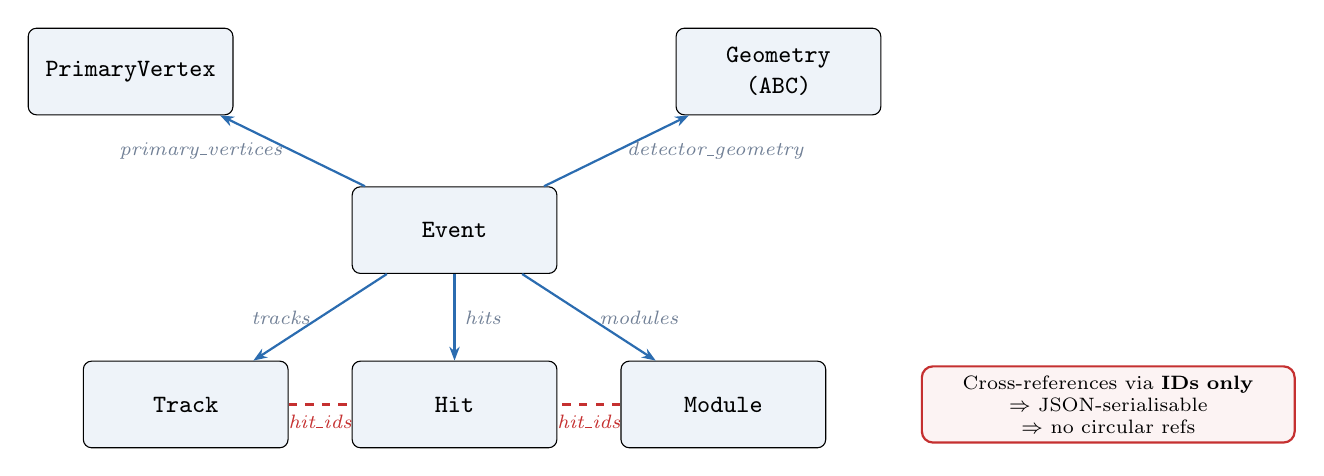
\begin{tikzpicture}[
      every node/.style={font=\small},
      box/.style={draw, rounded corners=3pt, fill=lhcbblue!8,
                  minimum width=2.6cm, minimum height=1.1cm,
                  align=center, font=\small\ttfamily},
      arr/.style={-{Stealth[length=5pt]}, thick, lhcbblue},
      note/.style={font=\scriptsize\itshape, text=lhcbgray},
    ]
    % Nodes
    \node[box] (event)  {Event};
    \node[box, below left=1.1cm and 0.8cm of event]  (track)  {Track};
    \node[box, below right=1.1cm and 0.8cm of event] (module) {Module};
    \node[box, below=1.1cm of event]                 (hit)    {Hit};
    \node[box, above right=0.9cm and 1.5cm of event] (geo)    {Geometry\\(ABC)};
    \node[box, above left=0.9cm and 1.5cm of event]  (pv)     {PrimaryVertex};

    % Arrows with labels
    \draw[arr] (event) -- (track)  node[midway, left, note] {tracks};
    \draw[arr] (event) -- (hit)    node[midway, right, note] {hits};
    \draw[arr] (event) -- (module) node[midway, right, note] {modules};
    \draw[arr] (event) -- (geo)    node[midway, right, note] {detector\_geometry};
    \draw[arr] (event) -- (pv)     node[midway, left, note] {primary\_vertices};

    % ID cross-refs (dashed)
    \draw[dashed, lhcbred, thick]
      (track) -- (hit) node[midway, below, note, text=lhcbred] {hit\_ids};
    \draw[dashed, lhcbred, thick]
      (module) -- (hit) node[midway, below, note, text=lhcbred] {hit\_ids};

    % Key change callout
    \node[draw=lhcbred, thick, rounded corners, fill=lhcbred!6,
          font=\scriptsize, text width=4.5cm, align=center,
          right=1.2cm of module]
      (note1) {Cross-references via \textbf{IDs only}\\%
               $\Rightarrow$ JSON-serialisable\\%
               $\Rightarrow$ no circular refs};
  \end{tikzpicture}
  \end{center}

  \vspace{-2pt}
  \footnotesize
  \textbf{Key change}: old code stored \emph{object references}
  (e.g.\ \texttt{Track.hits: list[Hit]}). New code stores
  \textbf{ID lists} (e.g.\ \texttt{Track.hit\_ids: list[int]}).
  Lookup is via \texttt{Event.get\_hit(hit\_id)}.
\end{frame}

% ------------------------------------------------------------------
\begin{frame}[fragile]{Dataclass Details}
  \begin{columns}[T]
    \begin{column}{0.48\textwidth}
      \textbf{Hit}
      \begin{lstlisting}
@dataclass
class Hit:
    hit_id:    HitID
    x:         float
    y:         float
    z:         float
    module_id: ModuleID
    track_id:  TrackID = -1
      \end{lstlisting}

      \textbf{Track}
      \begin{lstlisting}
@dataclass
class Track:
    track_id: TrackID
    pv_id:    PVID = 0
    hit_ids:  list[HitID]
      \end{lstlisting}
    \end{column}
    \begin{column}{0.48\textwidth}
      \textbf{Module}
      \begin{lstlisting}
@dataclass
class Module:
    module_id: ModuleID
    z:         float
    lx:        float   # half-width x
    ly:        float   # half-width y
    hit_ids:   list[int]
      \end{lstlisting}

      \textbf{Segment} {\scriptsize (reconstruction layer)}
      \begin{lstlisting}
@dataclass
class Segment:
    hit_start:  Hit
    hit_end:    Hit
    segment_id: SegmentID
    track_id:   TrackID = -1
    pv_id:      PVID  = -1
      \end{lstlisting}
    \end{column}
  \end{columns}

  \vspace{4pt}
  \footnotesize
  All type aliases (\texttt{HitID}, \texttt{ModuleID}, \ldots) are defined
  in \texttt{core/types.py} alongside the \texttt{SupportsPosition} protocol.
\end{frame}

% ------------------------------------------------------------------
\begin{frame}[fragile]{Geometry Hierarchy}
  \begin{columns}[T]
    \begin{column}{0.44\textwidth}
      \vspace{6pt}
      \begin{center}
      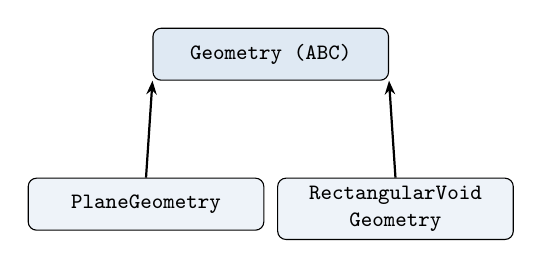
\begin{tikzpicture}[scale=0.88, every node/.style={transform shape},
          box/.style={draw, rounded corners=3pt, fill=lhcbblue!8,
                      minimum width=3.4cm, minimum height=0.75cm,
                      align=center, font=\small\ttfamily},
          arr/.style={-{Stealth[length=5pt]}, thick},
        ]
        \node[box, fill=lhcbblue!15, font=\small\ttfamily\bfseries]
              (base) {Geometry (ABC)};
        \node[box, below=1.4cm of base, xshift=-1.8cm]
              (plane) {PlaneGeometry};
        \node[box, below=1.4cm of base, xshift=1.8cm]
              (rect) {RectangularVoid\\Geometry};
        \draw[arr] (plane.north) -- (base.south west);
        \draw[arr] (rect.north)  -- (base.south east);
      \end{tikzpicture}
      \end{center}
      \vspace{4pt}
      \footnotesize
      \texttt{PlaneGeometry}: simple rectangular planes.\\
      \texttt{RectVoidGeometry}: planes with a beam-pipe hole.
    \end{column}
    \begin{column}{0.52\textwidth}
      \textbf{ABC contract}
      \begin{lstlisting}[basicstyle=\ttfamily\scriptsize]
class Geometry(ABC):
    @abstractmethod
    def __getitem__(idx) -> tuple
    @abstractmethod
    def __len__() -> int
    @abstractmethod
    def point_on_bulk(pos) -> bool
    @abstractmethod
    def get_z_positions() -> list
      \end{lstlisting}
    \end{column}
  \end{columns}
\end{frame}

% ======================================================================
\section{Pipeline Flow}
% ======================================================================

% ------------------------------------------------------------------
\begin{frame}{End-to-End Pipeline}
  \begin{center}
  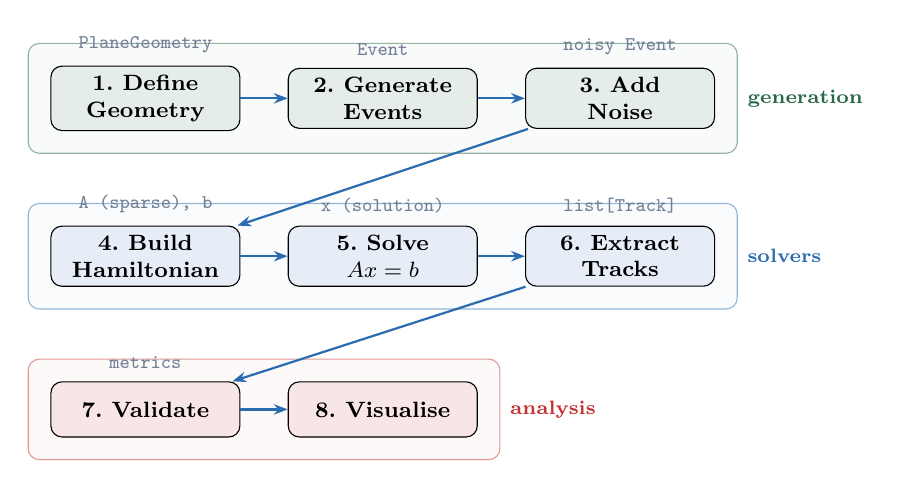
\begin{tikzpicture}[
      node distance=0.5cm and 0.6cm,
      stage/.style={draw, rounded corners=4pt, minimum width=2.4cm,
                    minimum height=0.7cm, align=center,
                    font=\footnotesize\bfseries},
      data/.style={font=\scriptsize\ttfamily, text=lhcbgray},
      arr/.style={-{Stealth[length=5pt]}, thick, lhcbblue},
    ]
    % Row 1 — generation (green)
    \node[stage, fill=lhcbgreen!12] (geo)
      {1.\ Define\\Geometry};
    \node[stage, fill=lhcbgreen!12, right=0.6cm of geo] (gen)
      {2.\ Generate\\Events};
    \node[stage, fill=lhcbgreen!12, right=0.6cm of gen] (noise)
      {3.\ Add\\Noise};

    % Row 2 — solvers (blue), below row 1
    \node[stage, fill=lhcbblue!12, below=1.2cm of geo] (ham)
      {4.\ Build\\Hamiltonian};
    \node[stage, fill=lhcbblue!12, right=0.6cm of ham] (solve)
      {5.\ Solve\\$Ax = b$};
    \node[stage, fill=lhcbblue!12, right=0.6cm of solve] (reco)
      {6.\ Extract\\Tracks};

    % Row 3 — analysis (red), below row 2
    \node[stage, fill=lhcbred!12, below=1.2cm of ham] (val)
      {7.\ Validate};
    \node[stage, fill=lhcbred!12, right=0.6cm of val] (plot)
      {8.\ Visualise};

    % Arrows — across rows
    \draw[arr] (geo)   -- (gen);
    \draw[arr] (gen)   -- (noise);
    \draw[arr] (noise) -- (ham);     % down to row 2
    \draw[arr] (ham)   -- (solve);
    \draw[arr] (solve) -- (reco);
    \draw[arr] (reco)  -- (val);     % down to row 3
    \draw[arr] (val)   -- (plot);

    % Data labels (outside the fit boxes)
    \node[data, above=1pt of geo]    {PlaneGeometry};
    \node[data, above=1pt of gen]    {Event};
    \node[data, above=1pt of noise]  {noisy Event};
    \node[data, above=1pt of ham]    {A (sparse), b};
    \node[data, above=1pt of solve]  {x (solution)};
    \node[data, above=1pt of reco]   {list[Track]};
    \node[data, above=1pt of val]    {metrics};

    % Layer boxes — each row is its own group, no overlap
    \begin{scope}[on background layer]
      \node[draw=lhcbgreen!50, fill=lhcbgreen!3, rounded corners,
            fit=(geo)(gen)(noise), inner sep=8pt,
            label={[font=\scriptsize\bfseries\color{lhcbgreen}]right:generation}] {};
      \node[draw=lhcbblue!50, fill=lhcbblue!3, rounded corners,
            fit=(ham)(solve)(reco), inner sep=8pt,
            label={[font=\scriptsize\bfseries\color{lhcbblue}]right:solvers}] {};
      \node[draw=lhcbred!50, fill=lhcbred!3, rounded corners,
            fit=(val)(plot), inner sep=8pt,
            label={[font=\scriptsize\bfseries\color{lhcbred}]right:analysis}] {};
    \end{scope}
  \end{tikzpicture}
  \end{center}

  \vspace{2pt}
  \footnotesize
  Each stage only depends on the \textbf{data objects} produced by the
  previous stage — never on the \emph{generator} class itself.
\end{frame}

% ------------------------------------------------------------------
\begin{frame}[fragile]{Pipeline — Code Sketch}
\begin{lstlisting}[basicstyle=\ttfamily\scriptsize]
# 1. Geometry
geo = PlaneGeometry(module_id=list(range(26)),
        lx=[50.0]*26, ly=[50.0]*26,
        z=[i * 55.0 for i in range(26)])
# 2-3. Generation + noise
gen = StateEventGenerator(detector_geometry=geo,
        theta_max=0.40, phi_max=0.30,
        collision_noise=0.01, measurement_error=0.02,
        events=1, n_particles=[8])
gen.generate_random_primary_vertices({'z': 50.0})
gen.generate_particles([[{'type':'MIP','mass':139.6,'q':1}]*8])
event       = gen.generate_complete_events()
noisy_event = gen.make_noisy_event(drop_rate=0.05,
                                   ghost_rate=0.10)
# 4. Hamiltonian
ham = SimpleHamiltonian(epsilon=0.02, gamma=1.5,
                         delta=1.0, theta_d=0.01)
A, b = ham.construct_hamiltonian(gen, convolution=False)

# 5. Solve
x = ham.solve_classicaly()    # or solve_direct(A, b)

# 6. Reconstruct
reco_tracks = get_tracks(ham, x, gen, threshold=0.5)

# 7-8. Validate & plot
validator = EventValidator(event, reco_tracks)
_, metrics = validator.match_tracks(purity_min=0.75)
fig = plot_event_3d(event, show_modules=True)
\end{lstlisting}
\end{frame}

% ======================================================================
\section{Key Differences}
% ======================================================================

% ------------------------------------------------------------------
\begin{frame}{Old vs.\ New: At a Glance}
  \scriptsize
  \renewcommand{\arraystretch}{1.15}
  \begin{center}
  \begin{tabular}{@{} l @{\hspace{6pt}} p{4.4cm} @{\hspace{6pt}} p{5.0cm} @{}}
    \toprule
    \textbf{Aspect}
      & \textbf{\color{lhcbred}Old}
      & \textbf{\color{lhcbgreen}New} \\
    \midrule
    Layout
      & Flat — 8 files, one folder
      & 4-layer tree: \texttt{core / generation / solvers / analysis} \\
    Generator
      & God class — factory \emph{\&} data store
      & Pure factory; returns \texttt{Event}; no mutable state \\
    Cross-refs
      & Object refs (\texttt{Track.hits})
      & ID lists (\texttt{Track.hit\_ids}) \\
    Segments
      & Stored on \texttt{Event} \& \texttt{Track}
      & Computed on-demand in \texttt{reconstruction/} \\
    Typing
      & Minimal; \texttt{dict} states; wildcard imports
      & \texttt{types.py} aliases, protocols, \texttt{py.typed} \\
    Visualisation
      & Embedded in \texttt{Event.plot\_segments()}
      & Standalone in \texttt{analysis/plotting/} \\
    Geometry
      & Defined alongside data classes
      & Separate sub-package with ABC contract \\
    Quantum
      & Not scaffolded
      & \texttt{solvers/quantum/} ready (HHL, 1-bit) \\
    \bottomrule
  \end{tabular}
  \end{center}
\end{frame}

% ------------------------------------------------------------------
\begin{frame}{Design Principles Applied}
  \begin{enumerate}
    \item \textbf{Single Responsibility} \\
          Each class does one thing:
          \texttt{Hit} stores a measurement,
          \texttt{Geometry} defines acceptance,
          \texttt{EventValidator} computes metrics.

    \item \textbf{Dependency Inversion} \\
          Solvers depend on the \texttt{Geometry} ABC — not on a
          concrete \texttt{PlaneGeometry}.

    \item \textbf{Open–Closed} \\
          Adding a new geometry (e.g.\ \texttt{PixelGeometry}) means
          subclassing \texttt{Geometry} and implementing four methods —
          no changes to downstream code.

    \item \textbf{Separation of Concerns} \\
          Plotting lives in \texttt{analysis/plotting/},
          data lives in \texttt{generation/entities/},
          solving lives in \texttt{solvers/}.

    \item \textbf{Serialisability} \\
          All cross-references use integer IDs so the full
          \texttt{Event} round-trips through JSON.
  \end{enumerate}
\end{frame}

% ======================================================================
\section{Segments: On-Demand Construction}
% ======================================================================

% ------------------------------------------------------------------
\begin{frame}[fragile]{Why Segments Are Not Stored}
  \begin{columns}[T]
    \begin{column}{0.46\textwidth}
      \textbf{\color{lhcbred}Old approach}
      \begin{itemize}
        \item \texttt{Event.segments} and \texttt{Track.segments}
              stored pre-computed segments
        \item Duplicated data (same info derivable from hits)
        \item Complicated serialisation
        \item Tight coupling to the generation phase
      \end{itemize}
    \end{column}
    \begin{column}{0.50\textwidth}
      \textbf{\color{lhcbgreen}New approach}
      \begin{itemize}
        \item Segments created \emph{on-demand} by\\
              \texttt{Hamiltonian.construct\_hamiltonian()}
        \item Live only in the reconstruction layer
        \item No duplication, no serialisation burden
        \item Different Hamiltonians can define different
              segment-building strategies
      \end{itemize}

      \begin{lstlisting}[basicstyle=\ttfamily\tiny]
# Segment built from two consecutive hits
seg = Segment(
    hit_start=hit_a,
    hit_end=hit_b,
    segment_id=next_id,
    track_id=-1   # unknown until reco
)
      \end{lstlisting}
    \end{column}
  \end{columns}
\end{frame}

% ======================================================================
\section{Solver Architecture}
% ======================================================================

% ------------------------------------------------------------------
\begin{frame}{Hamiltonian \& Solver Hierarchy}
  \begin{center}
  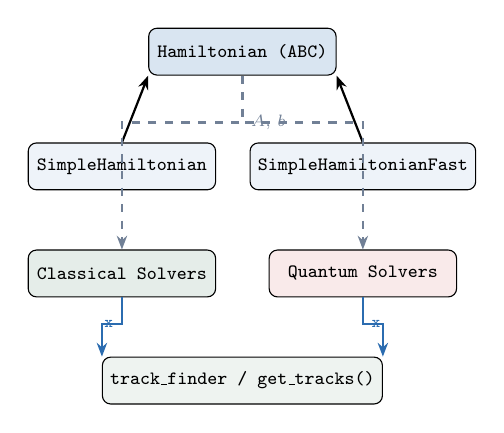
\begin{tikzpicture}[scale=0.85, every node/.style={transform shape},
      box/.style={draw, rounded corners=3pt, fill=lhcbblue!8,
                  minimum width=2.8cm, minimum height=0.7cm,
                  align=center, font=\footnotesize\ttfamily},
      arr/.style={-{Stealth[length=5pt]}, thick},
    ]
    % ── Row 1: Hamiltonian hierarchy ──
    \node[box, fill=lhcbblue!18, font=\footnotesize\ttfamily\bfseries]
          (base) {Hamiltonian (ABC)};
    \node[box, below=1.0cm of base, xshift=-1.8cm]
          (simple) {SimpleHamiltonian};
    \node[box, below=1.0cm of base, xshift=1.8cm]
          (fast)   {SimpleHamiltonianFast};
    \draw[arr] (simple.north) -- (base.south west);
    \draw[arr] (fast.north)   -- (base.south east);

    % ── Row 2: Solvers (both consume A,b → produce x) ──
    \node[box, fill=lhcbgreen!12, below=2.6cm of base, xshift=-1.8cm]
          (classical) {Classical Solvers};
    \node[box, fill=lhcbred!10, below=2.6cm of base, xshift=1.8cm]
          (quantum) {Quantum Solvers};

    % A,b arrows from Hamiltonian to both solver families
    \draw[arr, dashed, lhcbgray]
      (base.south) -- ++(0,-0.7) -| (classical.north)
      node[pos=0.0, right, font=\scriptsize\itshape] {$A,\,b$};
    \draw[arr, dashed, lhcbgray]
      (base.south) -- ++(0,-0.7) -| (quantum.north);

    % ── Row 3: Reconstruction ──
    \node[box, fill=lhcbgreen!8, below=4.2cm of base]
          (reco) {track\_finder / get\_tracks()};

    % x arrows from both solvers to reconstruction
    \draw[arr, lhcbblue]
      (classical.south) -- ++(0,-0.4) -| (reco.north west)
      node[pos=0.0, left, font=\scriptsize\ttfamily] {x};
    \draw[arr, lhcbblue]
      (quantum.south) -- ++(0,-0.4) -| (reco.north east)
      node[pos=0.0, right, font=\scriptsize\ttfamily] {x};
  \end{tikzpicture}
  \end{center}

  \vspace{2pt}
  \footnotesize
  \textbf{Classical}: \texttt{solve\_direct} (dense),
  \texttt{solve\_conjugate\_gradient} (sparse, iterative),
  \texttt{select\_solver} (auto-dispatch).\\
  \textbf{Quantum}: HHL and 1-bit HHL (OneBQF) — implemented with Qiskit.
\end{frame}

% ======================================================================
\section{Validation \& Reconstruction}
% ======================================================================

% ------------------------------------------------------------------
\begin{frame}{Non-Greedy Track Matching}
  \begin{columns}[T]
    \begin{column}{0.48\textwidth}
      \textbf{\color{lhcbred}Typical (greedy) approach}
      \begin{itemize}
        \item Match reconstructed tracks to truth tracks in
              arbitrary order
        \item First match ``wins'' — later, better matches
              may be blocked
        \item Can over-count clones and under-report efficiency
      \end{itemize}
    \end{column}
    \begin{column}{0.48\textwidth}
      \textbf{\color{lhcbgreen}New non-greedy matching}
      \begin{itemize}
        \item Rank \emph{all} candidate matches by a composite
              quality score: \texttt{purity $\times$ hit\_efficiency}
        \item Assign the globally best match first, then
              remove both tracks from the pool
        \item Repeat until no candidates exceed the
              \texttt{purity\_min} threshold
        \item Remaining unmatched reco tracks $\to$ ghosts;
              unmatched truth tracks $\to$ missed
      \end{itemize}
    \end{column}
  \end{columns}

  \vspace{6pt}
  \footnotesize
  \textbf{Result}: metrics are globally optimal — no match ordering
  artefacts. Implemented in \texttt{analysis/validation/validator.py}
  (\texttt{EventValidator.match\_tracks}).
\end{frame}

% ======================================================================
\section{Summary}
% ======================================================================

% ------------------------------------------------------------------
\begin{frame}{Summary}
  \begin{enumerate}
    \item \textbf{Modular package layout} with clear layer boundaries:\\
          \texttt{generation} $\to$ \texttt{solvers} $\to$ \texttt{analysis}

    \item \textbf{Clean dataclasses} (\texttt{Hit}, \texttt{Track}, \texttt{Module},
          \texttt{Event}) with ID-based cross-references and JSON round-tripping

    \item \textbf{Pluggable geometry} via an ABC; two implementations shipped

    \item \textbf{On-demand segments} — computed in the solver, not pre-stored

    \item \textbf{Non-greedy track matching} — globally optimal assignment,
          reliable efficiency and ghost-rate metrics

    \item \textbf{Quantum solvers} implemented and verified:
          HHL (cosine sim $>0.99$) and 1-BQF ($3.4{\times}$ shallower circuit)

    \item \textbf{Full type coverage} with aliases, protocols, and
          \texttt{py.typed}
  \end{enumerate}

\end{frame}

% ------------------------------------------------------------------
\begin{frame}{A Common Framework — Let's Collaborate}
  \begin{center}
    \large
    The goal of this work is the \textbf{start of a common framework}\\
    for quantum track-reconstruction research.
  \end{center}

  \vspace{6pt}
  \begin{itemize}
    \item \textbf{Shared codebase}: consistent event generation, Hamiltonian
          construction, and validation across groups
    \item \textbf{Easy to extend}: plug in new geometries, solvers, or
          analysis modules without touching the core
    \item \textbf{Reproducible benchmarks}: same metrics and matching
          for fair comparison of classical vs.\ quantum approaches
    \item \textbf{Open and pip-installable}: \texttt{pip install lhcb-velo-toy}
  \end{itemize}

  \vspace{8pt}
  \centering
  We would love to \textbf{work together} on this —\\
  contributions, feedback, and use cases are very welcome!
\end{frame}

% ------------------------------------------------------------------
\begin{frame}
  \centering
  \vspace{1.5cm}
  {\Huge\bfseries\color{lhcbblue} Thank you}

  \vspace{1cm}
  {\large Questions?}

  \vspace{1.5cm}
  \footnotesize
  \url{https://github.com/GeorgeWilliam1999/LHCb_VeLo_Toy_Model}
\end{frame}

\end{document}
